\section{Scrum} \label{sect:Scrum}

Scrum es un marco de trabajo iterativo e incremental para el desarrollo de proyectos y aplicaciones. El desarrollo esta organizado en ciclos de trabajo llamados \textit{Sprints} o iteraciones que son de duración fija y van sucediendo uno detrás de otro. Es importante destacar que sin importar que no se haya terminado el trabajo un \textit{Sprint} nunca se alarga \cite{DBLV09}. En el caso de Empresas TD las iteraciones tienen una duración de dos semanas.

\subsection{Roles en Scrum} 

Dentro de la metodología Scrum existen tres roles principales que debe ser cumplidos para la aplicación efectiva del proceso, estos son el el Dueño de Producto (DP), el Equipo y el ScrumMaster (SM). A continuación se describe cada rol, estas definiciones fueron extraídas de \cite{DBLV09}.

\begin{itemize}
\item El \textbf{Dueño del Producto} es el encargado de identificar las funcionalidades del producto y asignarles prioridad de acuerdo a las necesidades del negocio y debe revisar el resultado de cada iteración. Esta persona debe interactuar continuamente con el Equipo y tiene la autoridad final en el proyecto. En el caso de las pasantías el DP era el director general de Tuguia.de.
\item El \textbf{Equipo} es el encargado de construir el producto, en este caso el pasante. Debe poder autogestionarse y contar con un alto grado de autonomía y responsabilidad ya que al final de cada \textit{Sprint} debe poder tener un producto \textit{entregable}.
\item El \textbf{ScrumMaster} es el encargado de guiar al equipo y al DP en la aplicación y uso fructífero de Scrum, lo que hace es facilitar el proceso y ser un arbitro garante de la metológia y de que los demás actores ejecuten efectivamente su rol. Esta responsabilidad era de la gerencia e tecnología de Empresas TD.
\end{itemize} 

\subsection{El proceso de Scrum}

Como ya fue mencionado la metodología Scrum esta organizada en ciclos de trabajo que van ocurriendo uno tras otro. Estos ciclos están compuestos de actividades tal que se describe a continuación y como se muestra en la figura \ref{fig:scrum}. Las definiciones siguientes fueron obtenidas de \cite{DBLV09}.

\begin{figure}[h]
	\begin{center}
		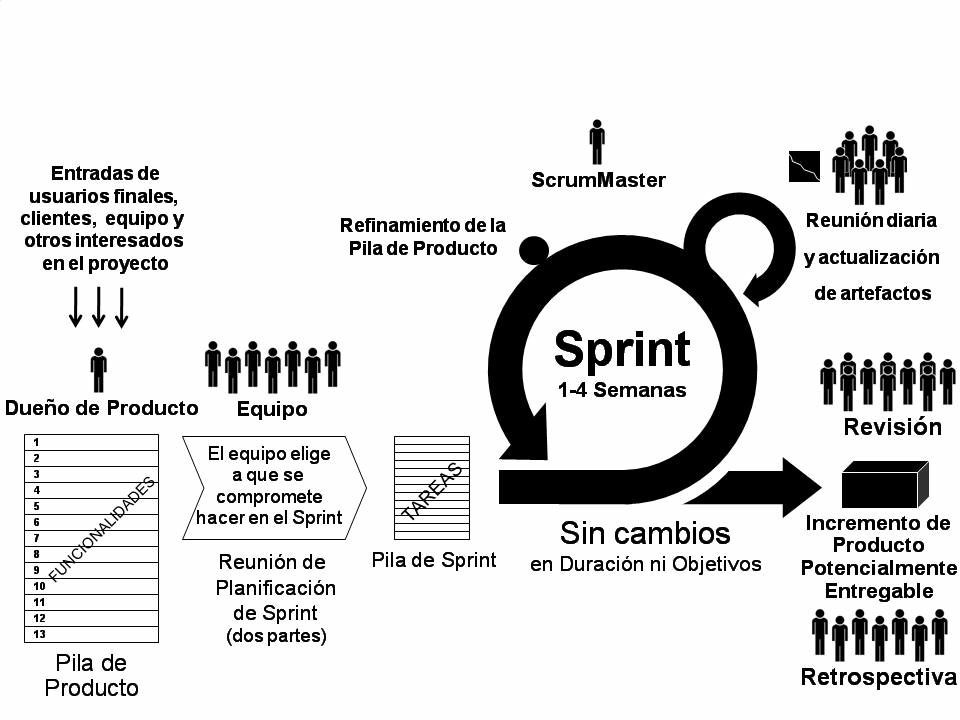
\includegraphics[scale=0.4]{imagenes/scrum.png}
	\end{center}
	\caption{
		\label{fig:scrum}
		Proceso Scrum \cite{DBLV09}
	}
\end{figure}

\begin{itemize}
\item \textbf{Planificación de la iteración:} La primera fase consiste en una reunión realizada al comienzo de la iteración donde al comienzo el DP presenta al equipo la lista de requisitos priorizada, se resuelven las dudas y se seleccionan los requisitos que se compromete a completar en la iteración, cada requisito es separado en tareas  yse estima la cantidad de esfuerzo en tiempo necesaria para completar cada una función del grado de dificultad de la misma.

\item \textbf{Ejecución de la iteración:} En esta fase más larga, en ésta se realiza el desarrollo del entregable. Durante esta fase, el equipo se reúne brevemente cada día para informar del progreso y dificultades. Cada miembro del equipo debe contestar únicamente las siguientes preguntas.
\begin{itemize}
\item ¿Qué ha hecho desde la última reunión?
\item ¿Qué tiene planificado hacer antes de la siguiente reunión?
\item ¿Qué impedimentos tiene o considera que va a tener?
\end{itemize}

\item \textbf{Inspección y adaptación:} Al finalizar el \textit{Sprint} se realiza una reunión, donde el equipo presenta el Dueño de la Aplicación los resultados obtenidos. En función de los resultados mostrados y de los cambios que haya habido en el contexto del proyecto, el DP realiza las adaptaciones necesarias de manera objetiva sobre la lista de requisitos. Por último el equipo debe analizar cómo ha sido su desempeño y cuales son los problemas que podrían impedirle progresar adecuadamente, tratando de mejorar de manera continua su productividad.

\end{itemize}








 
